%%%%%%%%%%%%%%%%%%%%%%%%%%%%%%%%%%%%%%%%%
% Wenneker Assignment
% LaTeX Template
% Version 2.0 (12/1/2019)
%
% This template originates from:
% http://www.LaTeXTemplates.com
%
% Authors:
% Vel (vel@LaTeXTemplates.com)
% Frits Wenneker
%
% License:
% CC BY-NC-SA 3.0 (http://creativecommons.org/licenses/by-nc-sa/3.0/)
% 
%%%%%%%%%%%%%%%%%%%%%%%%%%%%%%%%%%%%%%%%%

%----------------------------------------------------------------------------------------
%	PACKAGES AND OTHER DOCUMENT CONFIGURATIONS
%----------------------------------------------------------------------------------------

\documentclass[11pt]{scrartcl} % Font size
\usepackage{algorithmic}
%%%%%%%%%%%%%%%%%%%%%%%%%%%%%%%%%%%%%%%%%
% Wenneker Assignment
% Structure Specification File
% Version 2.0 (12/1/2019)
%
% This template originates from:
% http://www.LaTeXTemplates.com
%
% Authors:
% Vel (vel@LaTeXTemplates.com)
% Frits Wenneker
%
% License:
% CC BY-NC-SA 3.0 (http://creativecommons.org/licenses/by-nc-sa/3.0/)
% 
%%%%%%%%%%%%%%%%%%%%%%%%%%%%%%%%%%%%%%%%%

%----------------------------------------------------------------------------------------
%	PACKAGES AND OTHER DOCUMENT CONFIGURATIONS
%----------------------------------------------------------------------------------------

\usepackage{amsmath, amsfonts, amsthm} % Math packages

\usepackage{listings} % Code listings, with syntax highlighting

\usepackage[english]{babel} % English language hyphenation

\usepackage{graphicx} % Required for inserting images
\graphicspath{{Figures/}{./}} % Specifies where to look for included images (trailing slash required)

\usepackage{booktabs} % Required for better horizontal rules in tables

\numberwithin{equation}{section} % Number equations within sections (i.e. 1.1, 1.2, 2.1, 2.2 instead of 1, 2, 3, 4)
\numberwithin{figure}{section} % Number figures within sections (i.e. 1.1, 1.2, 2.1, 2.2 instead of 1, 2, 3, 4)
\numberwithin{table}{section} % Number tables within sections (i.e. 1.1, 1.2, 2.1, 2.2 instead of 1, 2, 3, 4)

\setlength\parindent{0pt} % Removes all indentation from paragraphs

\usepackage{enumitem} % Required for list customisation
\setlist{noitemsep} % No spacing between list items

%----------------------------------------------------------------------------------------
%	DOCUMENT MARGINS
%----------------------------------------------------------------------------------------

\usepackage{geometry} % Required for adjusting page dimensions and margins

\geometry{
	paper=a4paper, % Paper size, change to letterpaper for US letter size
	top=2.5cm, % Top margin
	bottom=3cm, % Bottom margin
	left=3cm, % Left margin
	right=3cm, % Right margin
	headheight=0.75cm, % Header height
	footskip=1.5cm, % Space from the bottom margin to the baseline of the footer
	headsep=0.75cm, % Space from the top margin to the baseline of the header
	%showframe, % Uncomment to show how the type block is set on the page
}

%----------------------------------------------------------------------------------------
%	FONTS
%----------------------------------------------------------------------------------------

\usepackage[utf8]{inputenc} % Required for inputting international characters
\usepackage[T1]{fontenc} % Use 8-bit encoding

\usepackage{fourier} % Use the Adobe Utopia font for the document

%----------------------------------------------------------------------------------------
%	SECTION TITLES
%----------------------------------------------------------------------------------------

\usepackage{sectsty} % Allows customising section commands

\sectionfont{\vspace{6pt}\centering\normalfont\scshape} % \section{} styling
\subsectionfont{\normalfont\bfseries} % \subsection{} styling
\subsubsectionfont{\normalfont\itshape} % \subsubsection{} styling
\paragraphfont{\normalfont\scshape} % \paragraph{} styling

%----------------------------------------------------------------------------------------
%	HEADERS AND FOOTERS
%----------------------------------------------------------------------------------------

\usepackage{scrlayer-scrpage} % Required for customising headers and footers

\ohead*{} % Right header
\ihead*{} % Left header
\chead*{} % Centre header

\ofoot*{} % Right footer
\ifoot*{} % Left footer
\cfoot*{\pagemark} % Centre footer
 % Include the file specifying the document structure and custom commands

%----------------------------------------------------------------------------------------
%	TITLE SECTION
%----------------------------------------------------------------------------------------

\title{	
	\normalfont\normalsize
	\textsc{Università degli Studi di Trieste}\\ % Your university, school and/or department name(s)
	\vspace{25pt} % Whitespace
	\rule{\linewidth}{0.5pt}\\ % Thin top horizontal rule
	\vspace{20pt} % Whitespace
	{\huge First FHPC Assignment}\\ % The assignment title
	\vspace{12pt} % Whitespace
	\rule{\linewidth}{2pt}\\ % Thick bottom horizontal rule
	\vspace{12pt} % Whitespace
}

\author{\LARGE Nicola Domenis} % Your name

\date{\normalsize\today} % Today's date (\today) or a custom date

\begin{document}

\maketitle % Print the title

%----------------------------------------------------------------------------------------
%	FIGURE EXAMPLE
%----------------------------------------------------------------------------------------

\section{Preview}
 
In this assignment we will present the following subjects:

\begin{itemize}
	\item the production of a parallel program code
	\item the graphs of the theoretical and real speedup of the code
	\item anything else
\end{itemize}


\begin{figure}[h] % [h] forces the figure to be output where it is defined in the code (it suppresses floating)
	\centering
	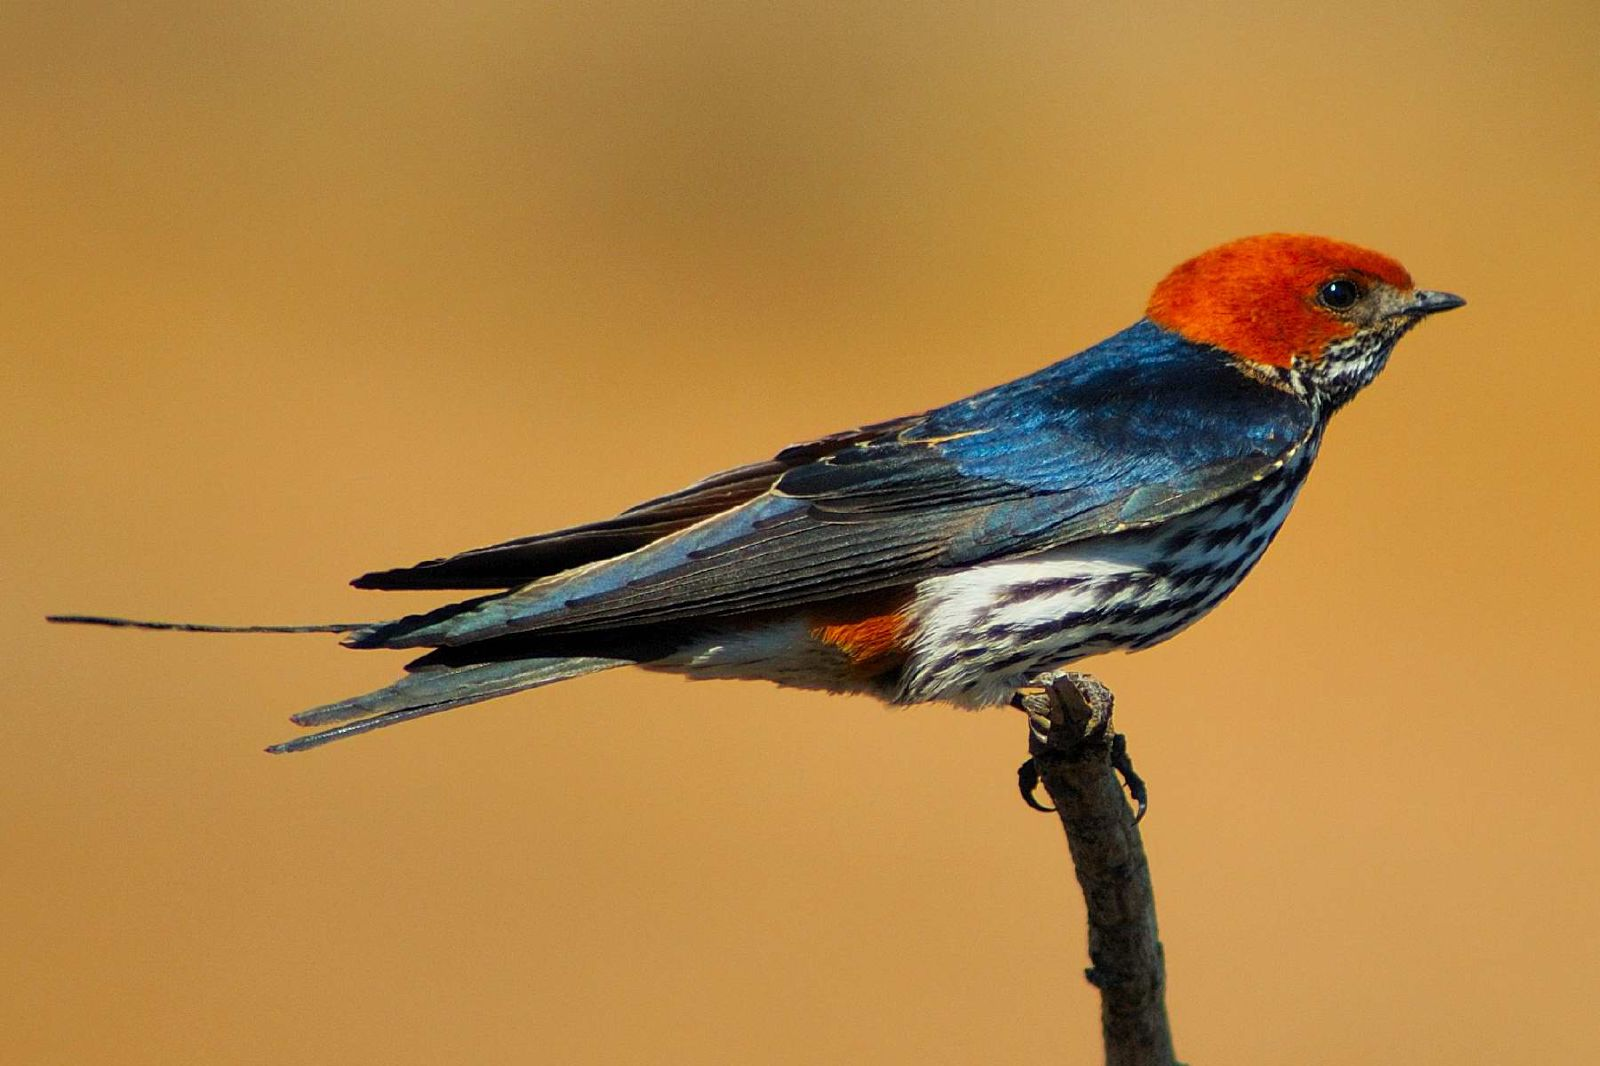
\includegraphics[width=0.5\columnwidth]{swallow.jpg} % Example image
	\caption{Photo of a parallel program}
\end{figure}

%------------------------------------------------
\section{section 0}
\subsection{Laptop theoretical peak performance}

We want to calculate the theoretical peak performance of our own portable computer by using the formula \textit{$theoretical peak performance$} $= clock_frequency x FLOPs x number of cores$.
We gather that $clock frequency = 2.90 Ghz$,$ FLOP = 16$ and $numberofcores = 2$ for our computer architecture,an intel i7 with a kaby lake microarchitecture; thus we compute $theoretical peak performance = 92.8 GFlops/s$
%Vect_size = dimensione di registro vettoriale stessa operaaxione nello stesso momento diviso dimensione double:andiamo a vedere se ci sono le sigle (mmx sse)128bit 2 double (avx avx2) 256bit 4 double (avx512)512bit 8 double
%primo fattore
%
%cercare FMA fused multiply addiction A = BxC+D  vec
%vector_size*2*#fma

%quanti cicli ci vogliono? pensiamo che sia 1 = 1*vector_size*2*#fma

%numero di operazioni in double precision

\begin{table}
	\centering
		\begin{tabular}{l| l| l| l| l| l| }
			&Your model&CPU&Frequency&Number of Cores&Peak Performance\\
			laptop& Asus F556U & Intel Core i7-7500 &$2.90$ GHz&2&92.8 GFLOPs/s
		\end{tabular}
	\label{Result}
\end{table}
\subsection{Smartphone theoretical peak performance}
We installed "`Mobile Linpack"' app and we run a few test. We report here some results,even on repeated trials: 

	\begin{tabular}{l| p{0.2\textwidth}| l |l| l|l }
		\hline
			&Model& Sustained performance&Matrix size&Peak performance&Memory\\
			\hline
			Cellphone&Samsung Galaxy XCover 4 &114,81 Mflops/s &250 &not calculated&16,00 GB\\
			& &145.53 Mflop/s&500& &\\
			& &157.5 Mflop/s&800& &\\
			& &201.32 Mflop/s&800& &\\
			& &155.93 Mflop/s&900& &\\
			& &109.88 Mflop/s&1000& &\\
			& &103.14 Mflop/s&2000& &\\
		\end{tabular}

\subsection{Laptops,smartphones and the top 500}
Let's check now whether our technologies would have competed with the Top500 supercomputers in the past:

	\begin{tabular}{l| p{0.2\textwidth}| l | p{0.3\textwidth}| p{0.3\textwidth}}
		\hline
			&Model&Performance&Top 500 year\& position&number 1 HPC system\\
			\hline
			Smartphone&Samsung Galaxy XCover 4 &201,32 Mflops/s &does not enter in the top500 of the first year of measurement, the 500th Supercomputer has an Rmax of 0.5 GFlops/s (equal to 2.4 times our smartphone peak performance)& Numerical Wind Tunnel,Fujitsu National Aerospace Laboratory of Japan is first in the year 1993 with a Rmax equal to 124.0 GFlops/s (equal to 616 times our cellphone's sustained peak performance)\\
			\hline
			Laptop&ASUS F556U&92.8 GFLOPs/s& 3rd position at nov 1993. Remains in the top 10 until nov 1996 & We have the same top position with a Rpeak equal to 235.8 GFlops/s(equal to 2.5 times our laptop's theoretical peak performance)\\
		\end{tabular}


%\begin{table}
	%\centering
		%\begin{tabular}{l| l| l |l| l| l}
			%&Model& Sustained performance&Matrix size&Peak performance&Memory\\
			%Cellphone&Samsung Galaxy XCover 4 &114,81 Mflops/s &250 &not calculated&16,00 GB
			%&&145.53 Mflop/s&500&&
			%&&157.5 Mflop/s&800&&
			%&&109.88 Mflop/s&1000&&
		%\end{tabular}
	%\label{Quick test parameters and results}
%\end{table}

%----------------------------------------------------------------------------------------
%	TEXT EXAMPLE
%----------------------------------------------------------------------------------------

\section{Section 1}

\subsection{Model for a serial and parallel summation of n numbers}
Here we discuss about modeling a simple program which consists of summing n numbers.
A simple pseudocode for the serial program would be:


\begin{algorithmic}

\STATE {Data:array $A[]$ of values}
\FOR{i from 1 to n} \STATE {sum = sum + A[i]} \ENDFOR
\RETURN{sum}
\end{algorithmic}

If we choose $T_{comp}$ as the time to compute a floating point operation we could calculate the total time of a serial computation as
$T_s = N * T_{comp}$,whereas the code simply computes N times the sum of two values.

For the parallel program we complicate a little the execution:

\begin{algorithmic}

\STATE {Data:array $A[]$ of values}
\STATE {Environment: p parallel processors}
\IF {Master process}

		\STATE{Read and Split $A[]$ into p subarrays $A_i[]$}
		\STATE{Send $p-1$ subarrays to the other $p-1$ processors}
		\FOR{i from $1$ to n/p} \STATE {$sum_i = sum_i + A_i[i]$} \ENDFOR
		\STATE{Collect the resulting $p-1$ values $sum_i$ from the processors}
		\FOR{i from $1$ to p} \STATE {$sum = sum + sum_i$} \ENDFOR
\ENDIF
\IF {Slave process}
	\STATE{Receive subarrays $A_i[]$ from the Master process}
	\FOR{i from 1 to n/p} \STATE {$sum_i = sum_i + A_i[i]$} \ENDFOR
	\STATE{Send $sum_i$ back to the Master process}
\ENDIF
\RETURN{sum}
\end{algorithmic}

If we define the times $T_{read}$ to indicate the time needed to read a variable,and $T_{comm}$ to indicate the time needed to communicate a variable, we can deduce the theoretical execution time of the model:
\  
\begin{algorithmic}
		\STATE{Read and Split $A[]$ into p subarrays $A_i[]$}
		\STATE{EXECUTION TIME: $T_{read}$
\end{algorithmic}
\ 
\begin{algorithmic}
		\STATE{Send $p-1$ subarrays to the other $p-1$ processors}
		\STATE{EXECUTION TIME: $T_{comm}*(p-1)$}
\end{algorithmic}
\ 

\begin{algorithmic}

\FOR{i from $1$ to n/p} \STATE {$sum_i = sum_i + A_i[i]$} \ENDFOR
\STATE{EXECUTION TIME: $p+n/p * T_{comp}=n*T_{comp}$}
\STATE{Notice that this is a parallel execution, the subarrays are added inside each processor}	
\end{algorithmic}

\ 
\begin{algorithmic}
\STATE{Send $sum_i$ back to the Master process}
\STATE{EXECUTION TIME: (p-1)*$T_{comm}$}
\end{algorithmic}

\begin{algorithmic}
		\FOR{i from $1$ to p} \STATE {$sum = sum + sum_i$} \ENDFOR
		\STATE{EXECUTION TIME: (p-1)*T_{comp}}
\end{algorithmic}

The total sum of the execution times gives $T_p = T_{read} + (p-1+1/n)*T_{comp}+2*T_{comm}(p-1)$
%----------------------------------------------

\subsection{Scalability of the Model}

Once we have the theoretical $T_p$ and $T_s$ we can calculate the Speedup given by the formula $$
%------------------------------------------------


%------------------------------------------------


%----------------------------------------------------------------------------------------
%	EQUATION EXAMPLES
%----------------------------------------------------------------------------------------

\section{Interpreting Equations}

\subsection{Identify the author of Equation \ref{eq:bayes} below and briefly describe it in English.}

\begin{align} 
	\label{eq:bayes}
	\begin{split}
		P(A|B) = \frac{P(B|A)P(A)}{P(B)}
	\end{split}					
\end{align}

Lorem ipsum dolor sit amet, consectetur adipiscing elit. Praesent porttitor arcu luctus, imperdiet urna iaculis, mattis eros. Pellentesque iaculis odio vel nisl ullamcorper, nec faucibus ipsum molestie. Sed dictum nisl non aliquet porttitor. Etiam vulputate arcu dignissim, finibus sem et, viverra nisl. Aenean luctus congue massa, ut laoreet metus ornare in. Nunc fermentum nisi imperdiet lectus tincidunt vestibulum at ac elit. Nulla mattis nisl eu malesuada suscipit.

%------------------------------------------------

\subsection{Try to make sense of some more equations.}

\begin{align} 
	\begin{split}
		(x+y)^3 &= (x+y)^2(x+y)\\
		&=(x^2+2xy+y^2)(x+y)\\
		&=(x^3+2x^2y+xy^2) + (x^2y+2xy^2+y^3)\\
		&=x^3+3x^2y+3xy^2+y^3
	\end{split}					
\end{align}

Lorem ipsum dolor sit amet, consectetuer adipiscing elit. 
\begin{align}
	A = 
	\begin{bmatrix}
		A_{11} & A_{21} \\
		A_{21} & A_{22}
	\end{bmatrix}
\end{align}
Aenean commodo ligula eget dolor. Aenean massa. Cum sociis natoque penatibus et magnis dis parturient montes, nascetur ridiculus mus. Donec quam felis, ultricies nec, pellentesque eu, pretium quis, sem.

%----------------------------------------------------------------------------------------
%	LIST EXAMPLES
%----------------------------------------------------------------------------------------

\section{Viewing Lists}

\subsection{Bullet Point List}

\begin{itemize}
	\item First item in a list 
		\begin{itemize}
		\item First item in a list 
			\begin{itemize}
			\item First item in a list 
			\item Second item in a list 
			\end{itemize}
		\item Second item in a list 
		\end{itemize}
	\item Second item in a list 
\end{itemize}

%------------------------------------------------

\subsection{Numbered List}

\begin{enumerate}
	\item First item in a list 
	\item Second item in a list 
	\item Third item in a list
\end{enumerate}

%----------------------------------------------------------------------------------------
%	TABLE EXAMPLE
%----------------------------------------------------------------------------------------

\section{Interpreting a Table}

\begin{table}[h] % [h] forces the table to be output where it is defined in the code (it suppresses floating)
	\centering % Centre the table
	\begin{tabular}{l l l}
		\toprule
		\textit{Per 50g} & \textbf{Pork} & \textbf{Soy} \\
		\midrule
		Energy & 760kJ & 538kJ\\
		Protein & 7.0g & 9.3g\\
		Carbohydrate & 0.0g & 4.9g\\
		Fat & 16.8g & 9.1g\\
		Sodium & 0.4g & 0.4g\\
		Fibre & 0.0g & 1.4g\\
		\bottomrule
	\end{tabular}
	\caption{Sausage nutrition.}
\end{table}

%------------------------------------------------

\subsection{The table above shows the nutritional consistencies of two sausage types. Explain their relative differences given what you know about daily adult nutritional recommendations.}

Lorem ipsum dolor sit amet, consectetur adipiscing elit. Praesent porttitor arcu luctus, imperdiet urna iaculis, mattis eros. Pellentesque iaculis odio vel nisl ullamcorper, nec faucibus ipsum molestie. Sed dictum nisl non aliquet porttitor. Etiam vulputate arcu dignissim, finibus sem et, viverra nisl. Aenean luctus congue massa, ut laoreet metus ornare in. Nunc fermentum nisi imperdiet lectus tincidunt vestibulum at ac elit. Nulla mattis nisl eu malesuada suscipit.

%----------------------------------------------------------------------------------------
%	CODE LISTING EXAMPLE
%----------------------------------------------------------------------------------------

\section{Reading a Code Listing}

\lstinputlisting[
	caption=Luftballons Perl Script., % Caption above the listing
	label=lst:luftballons, % Label for referencing this listing
	language=Perl, % Use Perl functions/syntax highlighting
	frame=single, % Frame around the code listing
	showstringspaces=false, % Don't put marks in string spaces
	numbers=left, % Line numbers on left
	numberstyle=\tiny, % Line numbers styling
	]{luftballons.pl}

%------------------------------------------------

\subsection{How many luftballons will be output by the Listing \ref{lst:luftballons} above?}

Aliquam arcu turpis, ultrices sed luctus ac, vehicula id metus. Morbi eu feugiat velit, et tempus augue. Proin ac mattis tortor. Donec tincidunt, ante rhoncus luctus semper, arcu lorem lobortis justo, nec convallis ante quam quis lectus. Aenean tincidunt sodales massa, et hendrerit tellus mattis ac. Sed non pretium nibh. Donec cursus maximus luctus. Vivamus lobortis eros et massa porta porttitor.

%------------------------------------------------

\subsection{Identify the regular expression in Listing \ref{lst:luftballons} and explain how it relates to the anti-war sentiments found in the rest of the script.}

Fusce varius orci ac magna dapibus porttitor. In tempor leo a neque bibendum sollicitudin. Nulla pretium fermentum nisi, eget sodales magna facilisis eu. Praesent aliquet nulla ut bibendum lacinia. Donec vel mauris vulputate, commodo ligula ut, egestas orci. Suspendisse commodo odio sed hendrerit lobortis. Donec finibus eros erat, vel ornare enim mattis et.

%----------------------------------------------------------------------------------------

\end{document}
